\interlude{Real-world concerns}

\SetNextBackground{\includegraphics[width=\paperwidth,page=13]{hpke-in-avionics-slide-designs}}
\begin{frame}{Sometimes, availability beats everything else}
  \begin{minipage}{.45\pagewidth}
    There is no fail-safe way to stop a plane.
    \\[1.3em] If your cipher depends on dropping packets, it won't encrypt pilot radio.
  \end{minipage}
\end{frame}

\SetNextBackground{}
\begin{frame}{Real-world Rosenpass: DoS resistance}
  \begin{columns}[]
    \begin{column}{.2\textwidth}
      % Somehow, I can not place the vrule after the graphic, hence the double reflectbox
      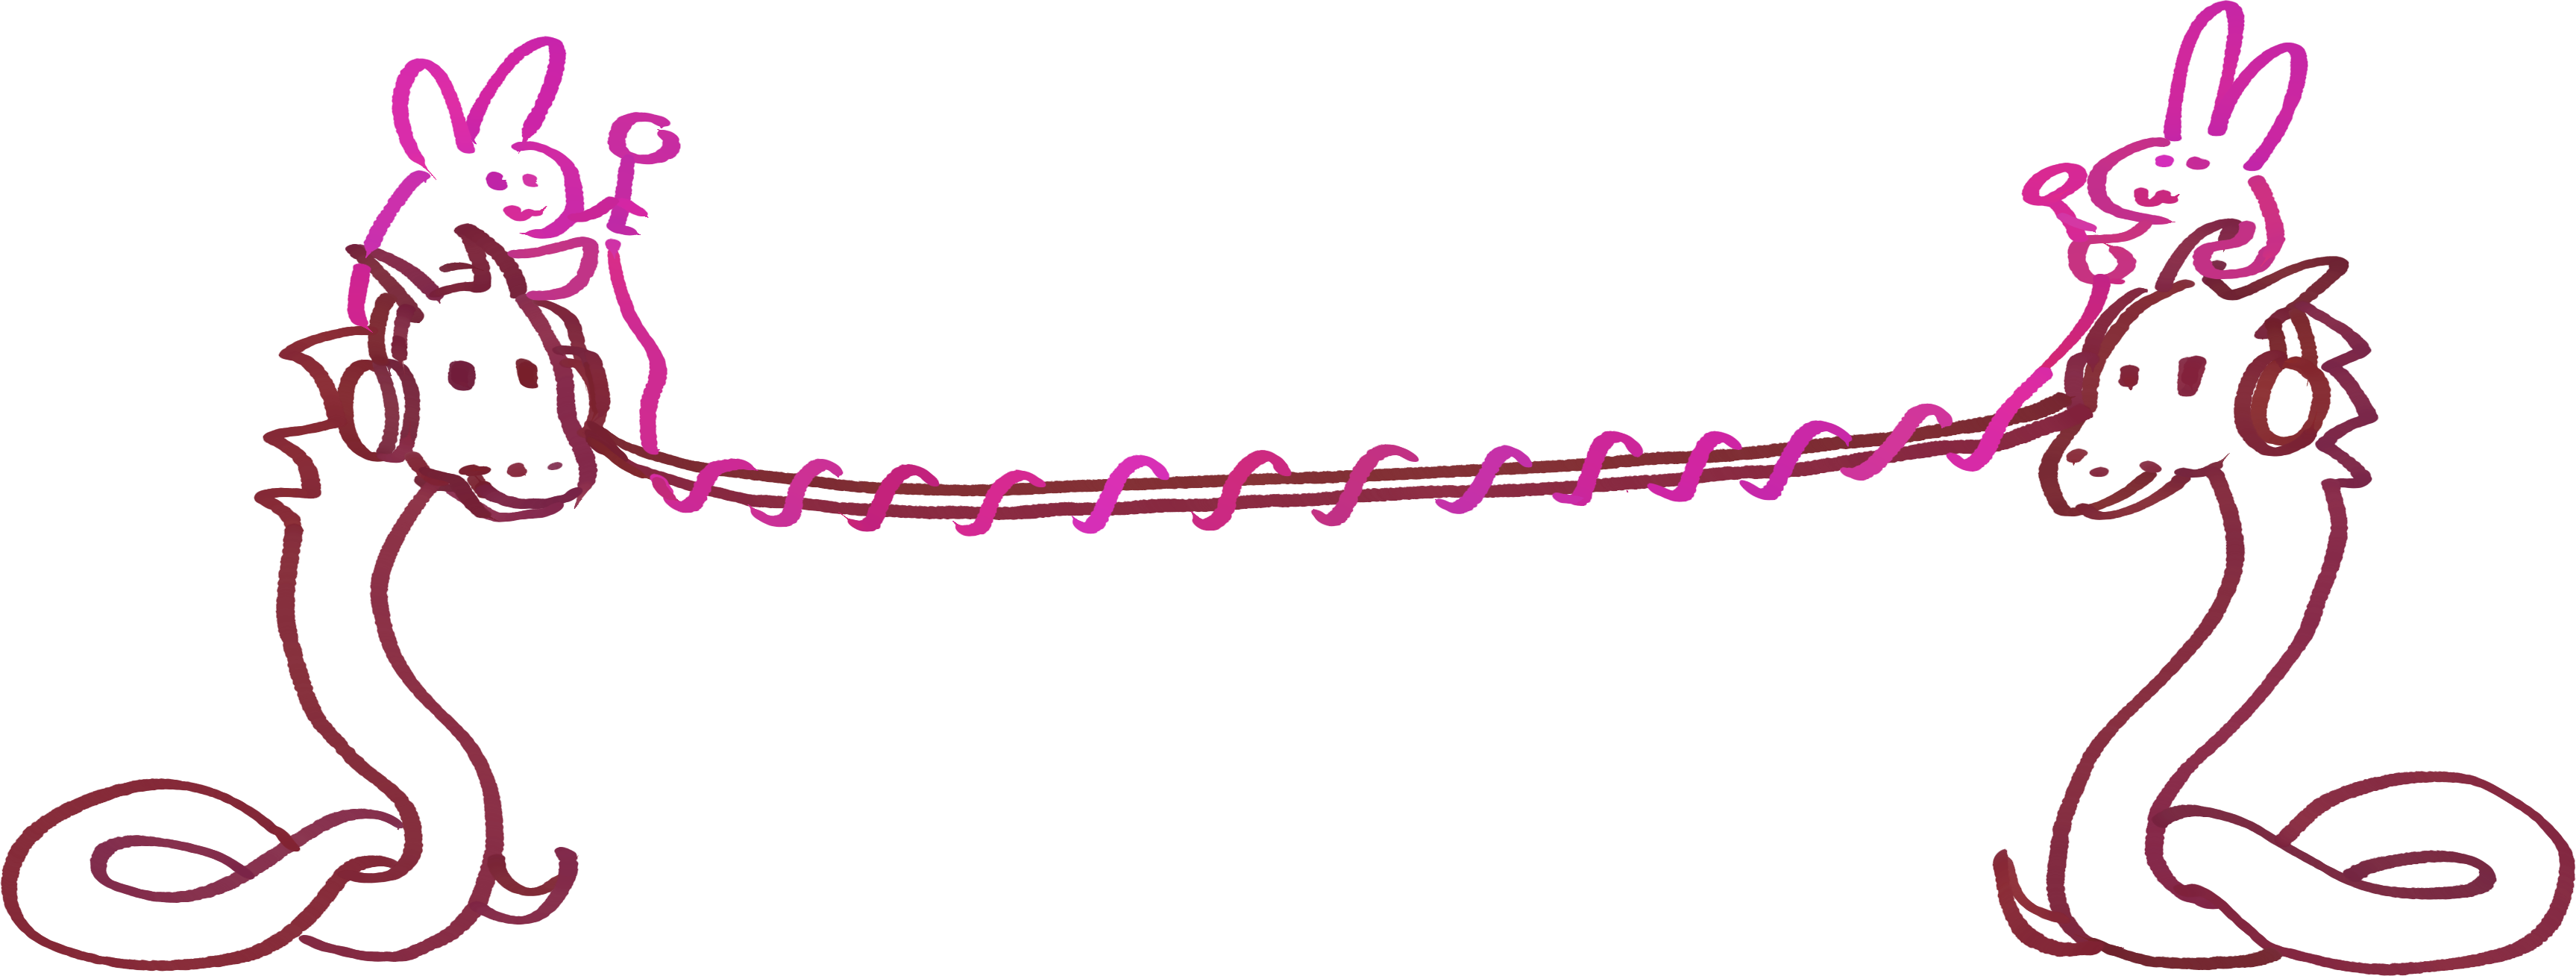
\includegraphics[width=\textwidth-.4pt,clip,trim=0 0 2300 0]{graphics/wireguard-and-rp-bunny-rose.png}\rule{.4pt}{.45\textheight}
      % \begin{minipage}[][.4pt]{.4pt}
      %   \rule{.4pt}{.35\textheight}
      % \end{minipage}
    \end{column}

    \begin{column}{.7\textwidth}
      \centering
      \begin{minipage}{\textwidth}
        \begin{itemize}
          \item Protocol-level DoS (\say{State Disruption Attacks})
          \item Memory-DoS (attacker-triggered allocations)
          \item CPU-exhaustion DoS
          \item DoS-Amplification (e.g. abusing DNS)
        \end{itemize}
      \end{minipage}
    \end{column}
    \begin{column}{.2\textwidth}
      \rule{.4pt}{.45\textheight}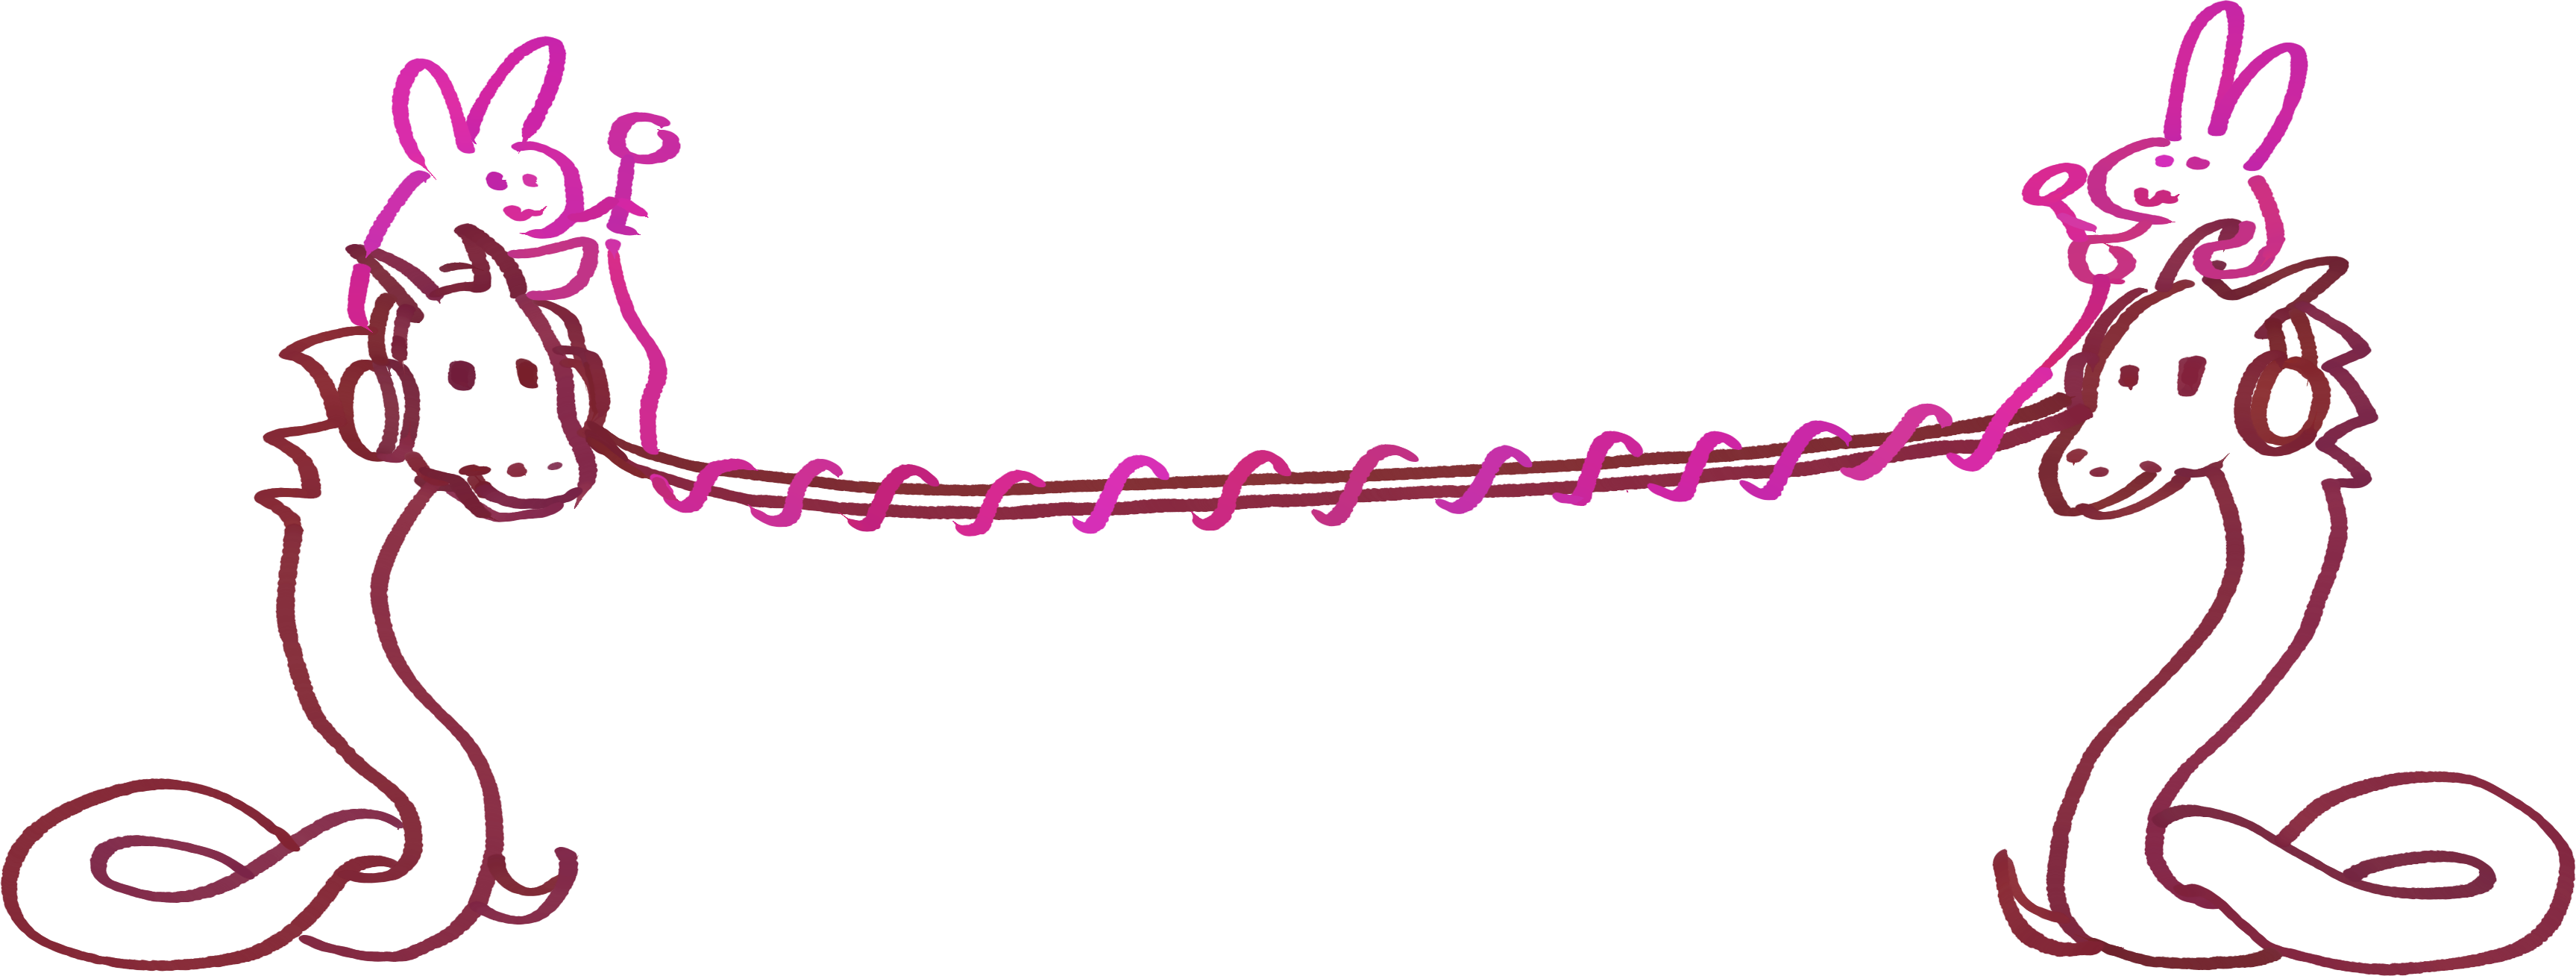
\includegraphics[width=\textwidth-.4pt,clip,trim=2300 0 0 0]{graphics/wireguard-and-rp-bunny-rose.png}
    \end{column}
  \end{columns}
\end{frame}

\SetNextBackground{\vspace{.5\pageheight}\begin{minipage}[T][5pt]{.6\pagewidth}~\end{minipage}\reflectbox{
\includegraphics[width=.7\pagewidth,trim=0 130 300 0,clip]{graphics/gray-hamster-eating-sunflower-seed.jpeg}}}
\begin{frame}{Real-world Rosenpass: Stealth}
  \begin{minipage}{.5\pagewidth}
    \centering
    The protocol should not respond to authentication.
    \\[1.3em] This prevents port-scanning.
    \\[1.3em] Rosenpass and WireGuard archieve this using symmetric pre-authentication.
    \\[1.3em] Breaking identity-hiding in the process.
  \end{minipage}
\end{frame}
